\documentclass[12pt, a4]{article}
\usepackage[english]{babel}
\usepackage[utf8x]{inputenc}
\usepackage{fullpage}
\usepackage{listings}
\usepackage{graphicx}
\usepackage{color}

%Syntax highlighting
\definecolor{blue-violet}{rgb}{0.54, 0.17, 0.89}
\definecolor{ao}{rgb}{0.0, 0.5, 0.0}
\definecolor{amaranth}{rgb}{0.9, 0.17, 0.31}
\definecolor{ballblue}{rgb}{0.13, 0.67, 0.8}
\definecolor{onyx}{rgb}{0.06, 0.06, 0.06}


\lstset{
  breaklines=true,                 % automatic line breaking only at whitespace
  captionpos=b,                    % sets the caption-position to bottom
  breakatwhitespace=false,
  keepspaces=true,
  numbers=left,
  numbersep=5pt,
  showspaces=false,
  showstringspaces=false,
  showtabs=false,
  tabsize=4,  
  backgroundcolor=\color{white},   % choose the background color
  commentstyle=\color{ao},    % comment style
  keywordstyle=\color{amaranth},    % keyword style
  stringstyle=\color{blue-violet},    % string literal style
  numberstyle=\tiny\color{ballblue},	   % number style
  basicstyle=\ttfamily\footnotesize\color{onyx} % size of fonts used for the code
}

%Document Header
\title{\textbf{Department of CSE\\SSN College of Engineering}}
\author{\textbf{Vishakan Subramanian - 18 5001 196 - Semester VII}}
\date{10 October 2021}

\begin{document}
\maketitle
\hrule
\section*{\center{UCS 1711 - Mobile Application Development Lab}}
\hrule
\bigskip

%Assignment Details
\subsection*{\center{\textbf{Exercise 8: SMS Message Application using Android}}}
\subsection*{\flushleft{Aim:}}
\begin{flushleft}

To develop a native application that can send an SMS to other phone numbers, and to display notifications upon reception of a new message.

\end{flushleft}

%Code
\newpage
\subsection*{\flushleft{Code - SMS: Main Activity:}}
\begin{flushleft}
\lstinputlisting[language = Java]{SMS/app/src/main/java/com/example/sms/MainActivity.java}
\end{flushleft}

%Code
\newpage
\subsection*{\flushleft{Code - SMS: Message Receiver:}}
\begin{flushleft}
\lstinputlisting[language = Java]{SMS/app/src/main/java/com/example/sms/MessageReceiver.java}
\end{flushleft}


%Code
\newpage
\subsection*{\flushleft{Code - SMS: Main Activity Layout:}}
\begin{flushleft}
\lstinputlisting[language = XML]{SMS/app/src/main/res/layout/activity_main.xml}
\end{flushleft}

%Code
\newpage
\subsection*{\flushleft{Code - SMS: Android Manifest XML:}}
\begin{flushleft}
\lstinputlisting[language = XML]{SMS/app/src/main/AndroidManifest.xml}
\end{flushleft}


%Output
\newpage
\subsection*{\flushleft{Output: Main Screen:}}
\begin{figure}[h]
\centering
\caption{Output: Main Screen.}
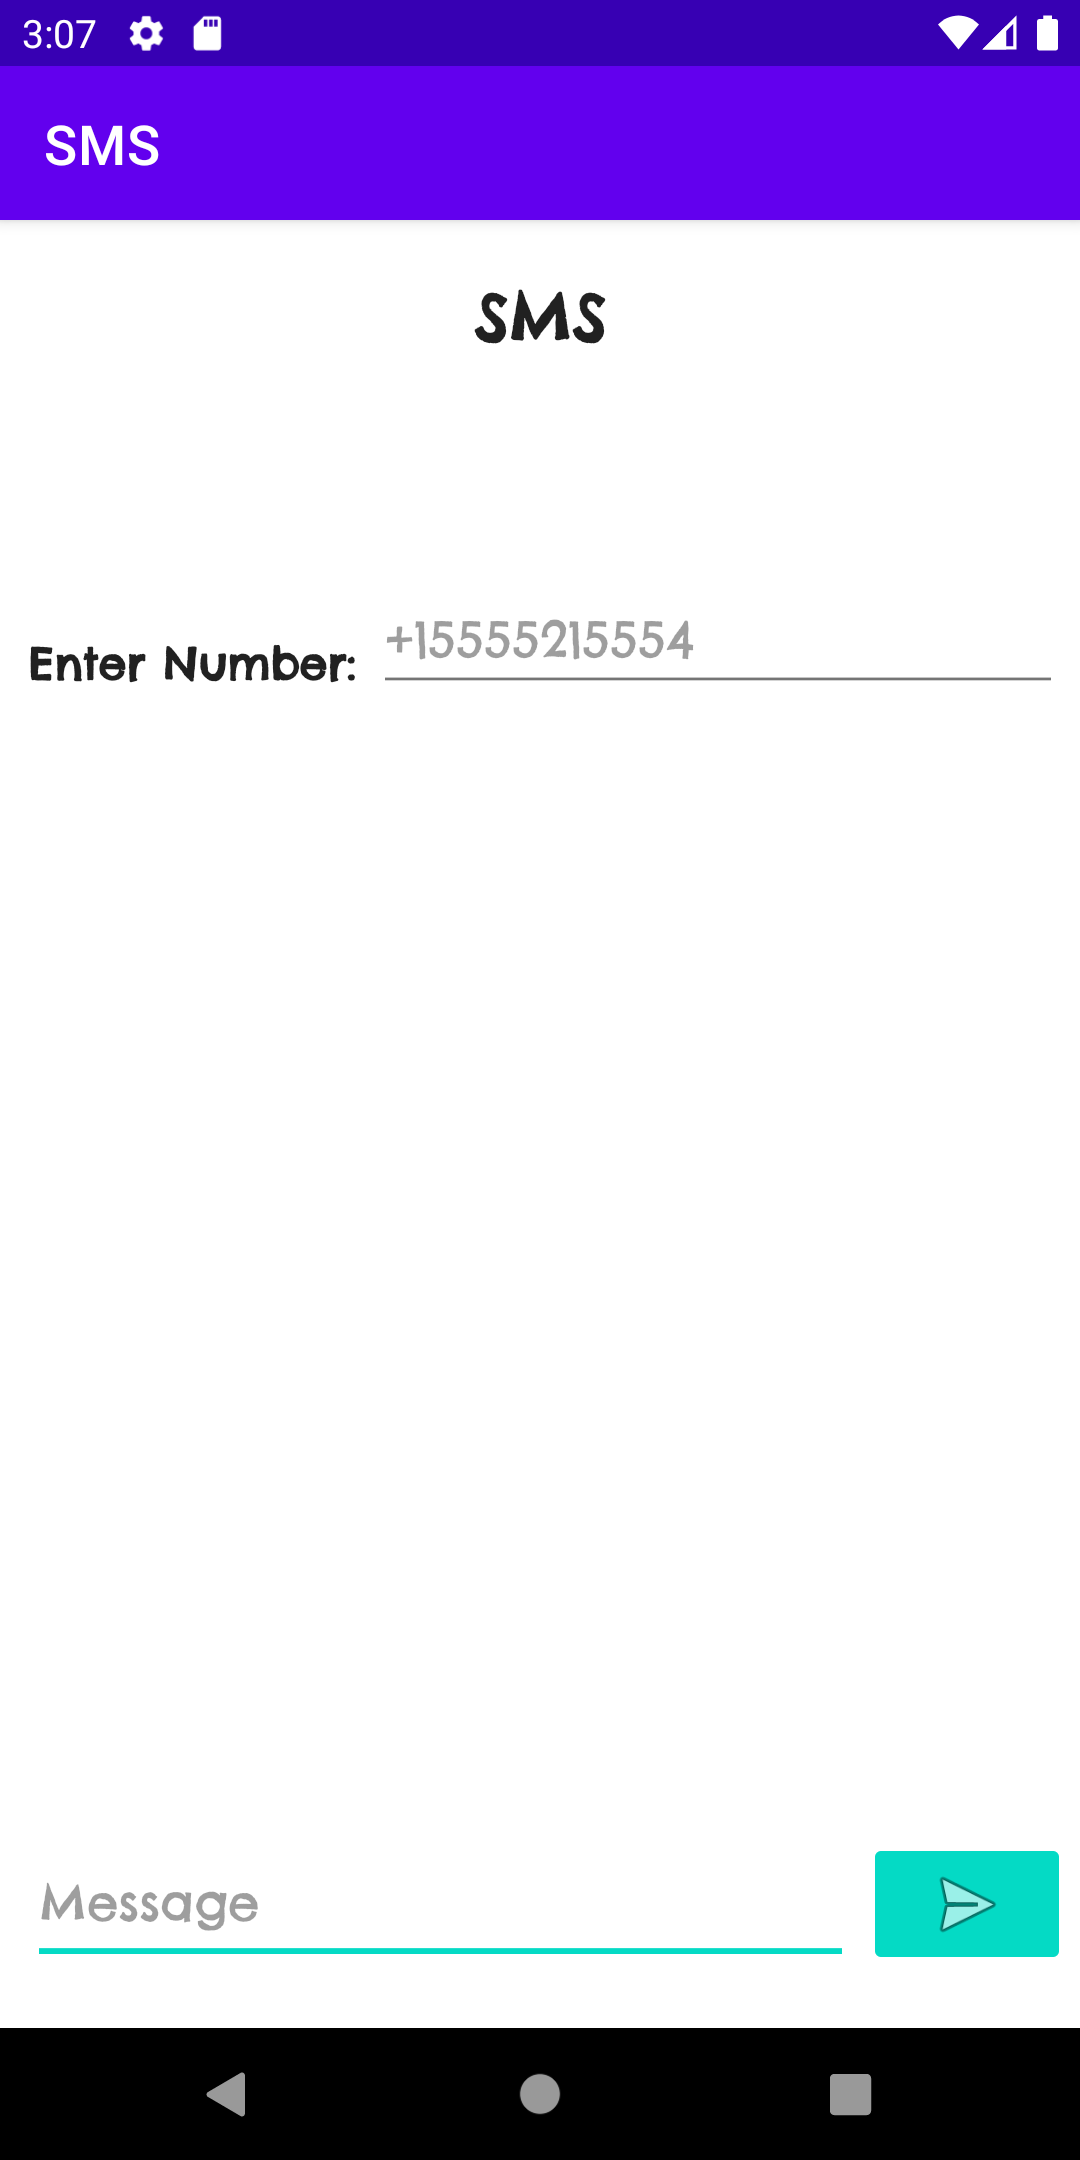
\includegraphics[height=15cm, width=7.3cm]{SMS/Screenshots/Output-1.png}
\end{figure}

%Output
\newpage
\subsection*{\flushleft{Output: SMS Sent \& Received:}}
\begin{figure}[h]
\centering
\caption{Output: SMS Sent \& Received.}
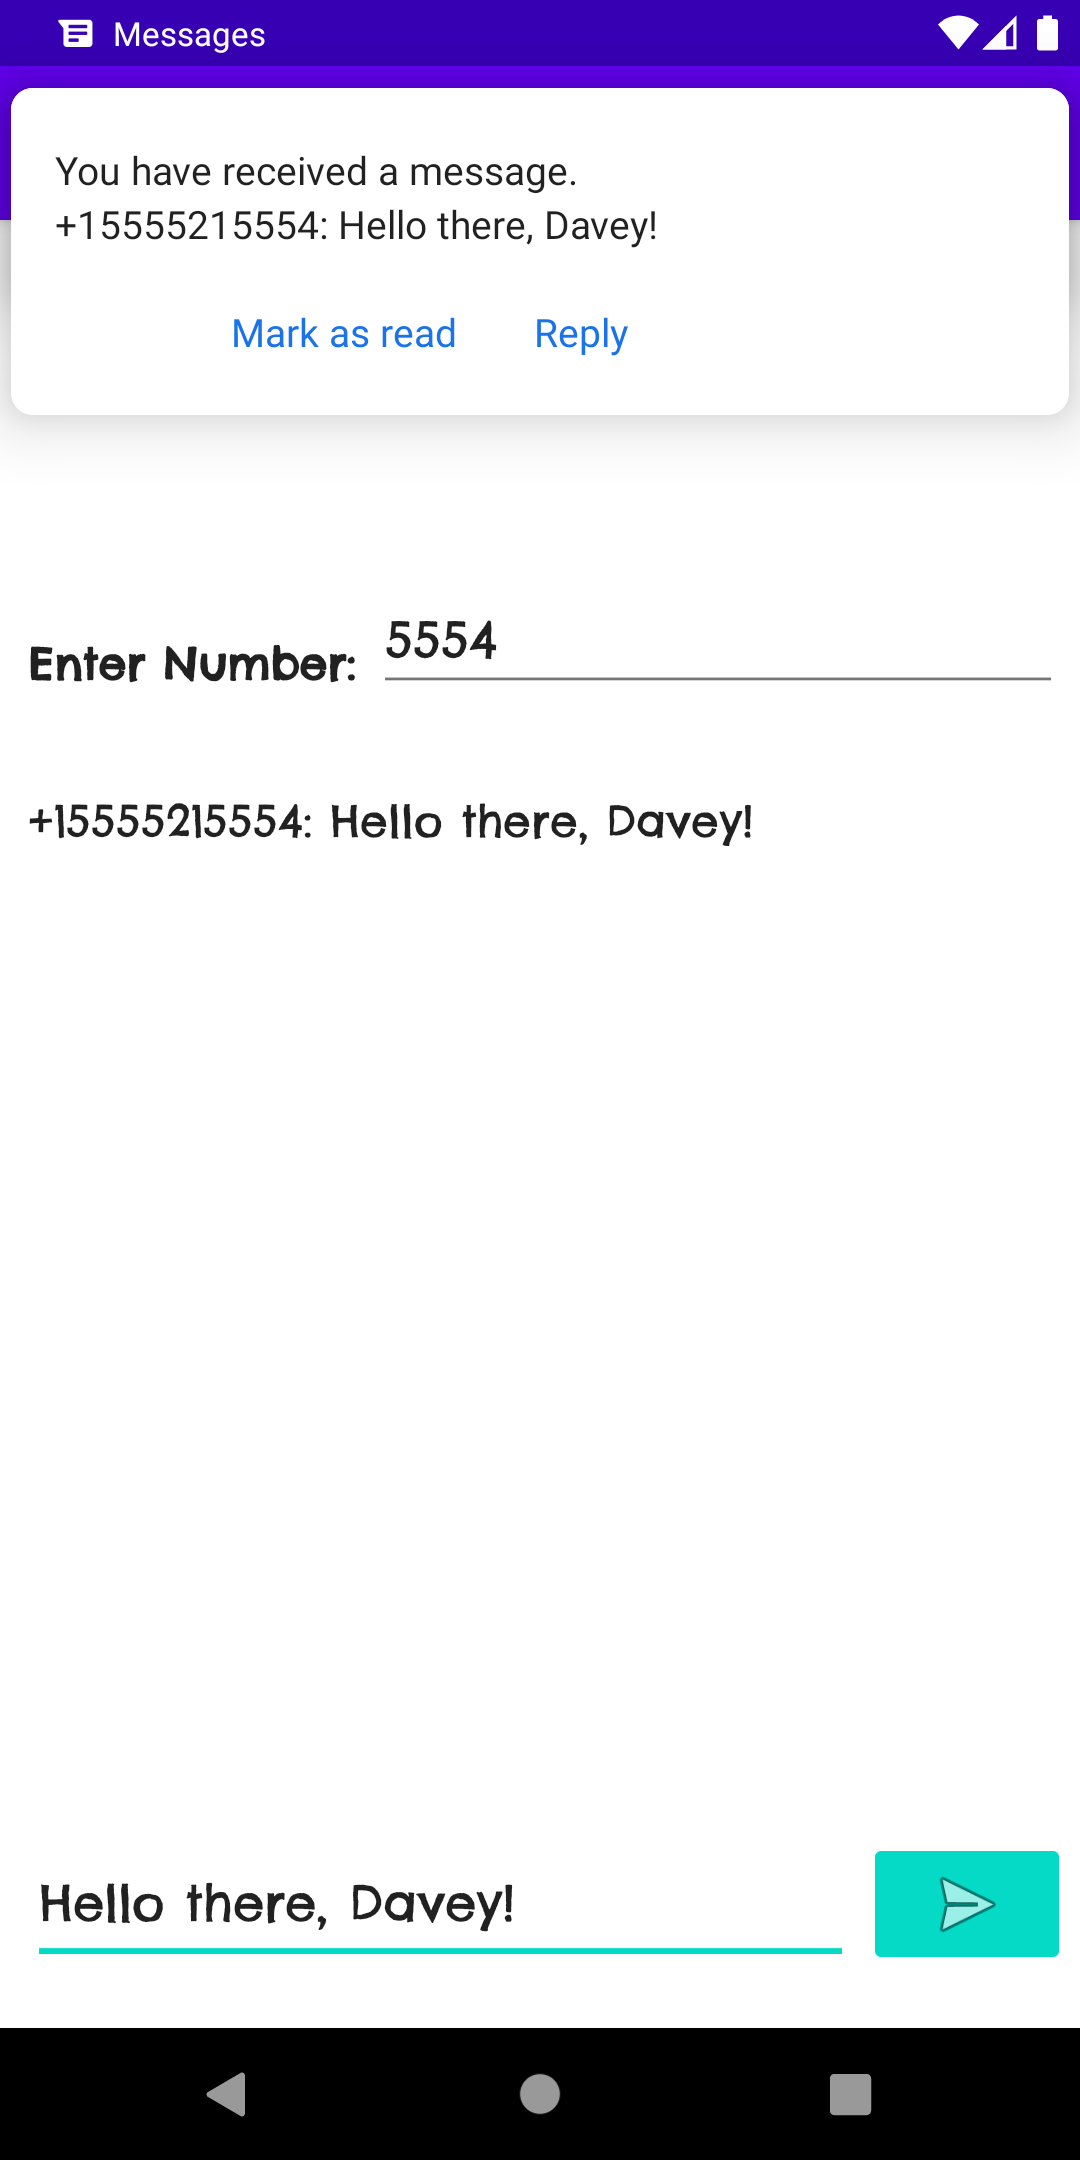
\includegraphics[height=15cm, width=7.3cm]{SMS/Screenshots/Output-2.png}
\end{figure}

%Output
\newpage
\subsection*{\flushleft{Output: SMS Notification:}}
\begin{figure}[h]
\centering
\caption{Output: SMS Notification.}
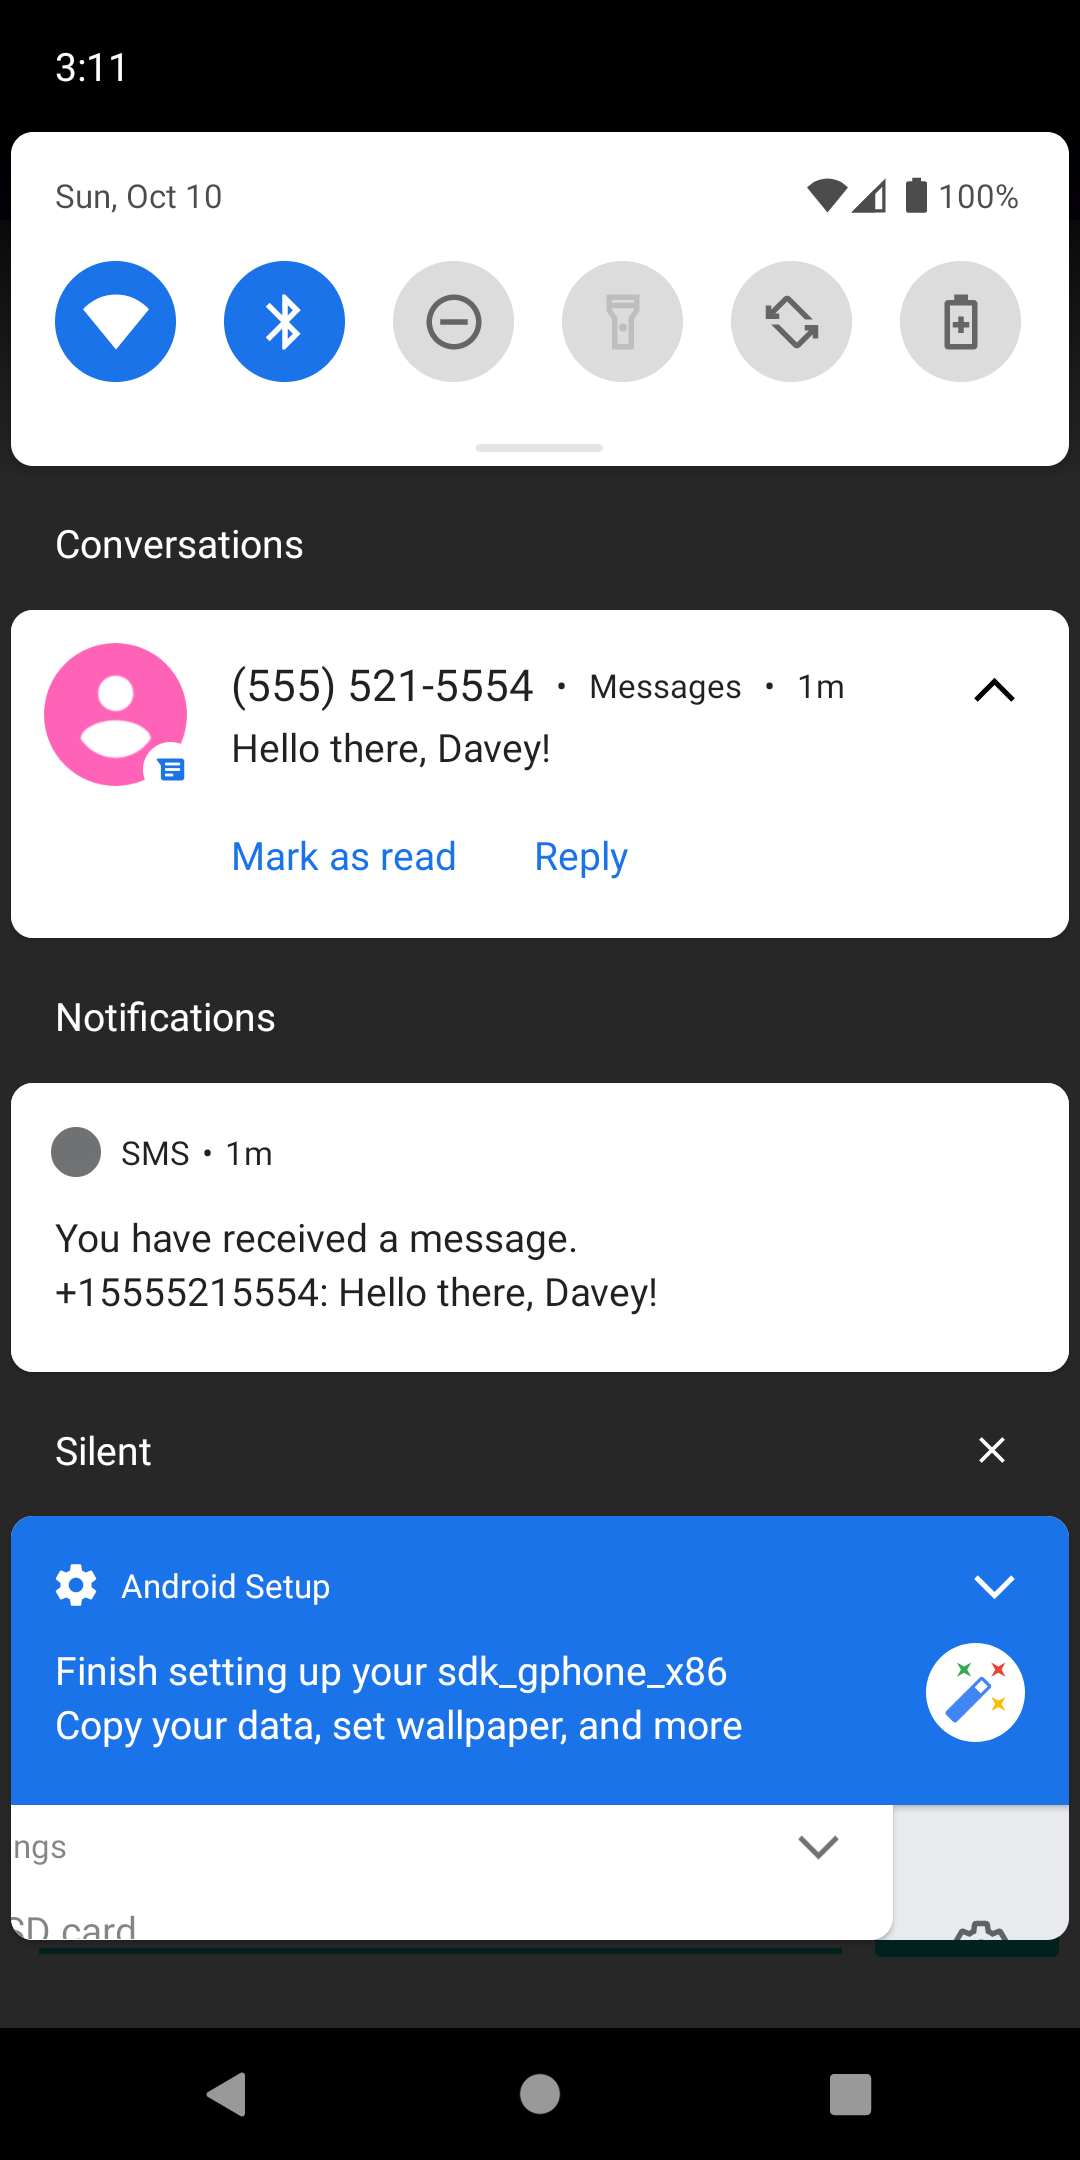
\includegraphics[height=15cm, width=7.3cm]{SMS/Screenshots/Output-3.png}
\end{figure}


%Learning Outcome
\newpage
\subsection*{\flushleft{Learning Outcome:}}
\begin{itemize}

\item I learnt to set permissions like \textbf{READ\_SMS, SEND\_SMS} etc. to enable SMS telephony services for the application.
\item I implemented methods to prompt the user to allow the SMS permissions to be given for the application.
\item I implemented a \textbf{BroadcastReceiver} class to take care of message reception handling.
\item I understood how to set a \textbf{ScrollView} and how to work with \textbf{LinearLayout}.
\item I learnt how to send a message using the \textbf{SmsManager} class.
\item I understood how to work with BroadcastReceiver and Intents. \item I learnt how to parse the received SMS messages using \textbf{Bundle} object as \textbf{PDUs} (Protocol Data Units)
\item I implemented a notification alert to the user upon reception of a message using the \textbf{NotificationCompat.Builder} and \textbf{NotificationManager} classes.
\item I learnt how to set the notification to a channel and how to notify using the manager using the notify() method.
\item I learnt how to send the received message from the MessageReceiver handler to the MainActivity using BroadcastReceiver and Intent, using \textbf{sendBroadcast()} method.
\end{itemize}


\end{document}